\documentclass{beamer}
%\documentclass[handout]{beamer}

\usepackage{xcolor}
\usepackage{amsmath}

\input ../macros.tex

\beamerdefaultoverlayspecification{<+->}

\definecolor{mathred}{RGB}{200,0,0}
\definecolor{mathcolor}{RGB}{200,0,0}
\newcommand{\redmath}[1]{\textcolor{mathred}{#1}}
\newcommand{\mathred}[1]{\textcolor{mathred}{#1}}
\mode<presentation>
{
  \usetheme{Montpellier}

  %\setbeamercovered{transparent}
  % or whatever (possibly just delete it)
}
\title{Dual Descent}

\begin{document}

\begin{small}

\begin{frame}
  \titlepage
{\bf Chapter 2 in Shai Shalev Shwartz / Online Learning and Online convex Optimization} 
\end{frame}

\begin{frame}{Follow-the-Regularized-Leader (FTRL)}
        \begin{equation*}
            \forall t, \quad \mathbf{w}_t = \arg\min_{\mathbf{w} \in S} \sum_{i=1}^{t-1} f_i(\mathbf{w}) + R(\mathbf{w})
        \end{equation*}
\begin{itemize}
  \item Regularizer controls length of weight vector -> changes from iteration to iteration.
  \item Each step requires solving a constrained minimization problem.
    \end{itemize}
\end{frame}

\begin{frame}{Review: Property of FoRel Algorithm}
\textbf{Lemma 2.3:}\\
Let $\mathred{w_1, w_2, \dots}$ be the sequence of vectors produced by the FoReL algorithm. Then, for all $\mathred{u \in S}$, we have:
\begin{equation*}
\mathred{\sum_{t=1}^{T} (f_t(w_t) - f_t(u)) \leq R(u) - R(w_1) + \sum_{t=1}^{T} (f_t(w_t) - f_t(w_{t+1}))}
\end{equation*}
\end{frame}

\iffalse
\begin{frame}{Proof of Lemma 2.3}
\textbf{Proof:}\\
Running FoReL on $\mathred{f_1, \dots, f_T}$ is equivalent to running FTL on $\mathred{f_0, f_1, \dots, f_T}$ where $\mathred{f_0 = R}$. Using Lemma 2.1, we have:
\begin{equation*}
\mathred{\sum_{t=0}^{T} (f_t(w_t) - f_t(u)) \leq \sum_{t=0}^{T} (f_t(w_t) - f_t(w_{t+1}))}
\end{equation*}

Rearranging terms and using $\mathred{f_0 = R}$, we obtain:
\begin{equation*}
\mathred{\sum_{t=1}^{T} (f_t(w_t) - f_t(u)) \leq R(u) - R(w_1) + \sum_{t=1}^{T} (f_t(w_t) - f_t(w_{t+1}))}
\end{equation*}
\end{frame}
\fi

\begin{frame}{Review: One step of Gradient Descent using strongly convex regularizer}
\textbf{Lemma 2.10:}\\
Let $\mathred{R : S \to \mathbb{R}}$ be a $\mathred{\sigma}$-strongly-convex function over $S$ with respect to a norm $\mathred{\|\cdot\|}$. Let $\mathred{w_1, w_2, \dots}$ be the predictions of the FoReL algorithm. Then, for all $t$, if $\mathred{f_t}$ is $\mathred{L_t}$-Lipschitz with respect to $\mathred{\|\cdot\|}$, we have:
\begin{equation*}
\mathred{f_t(w_t) - f_t(w_{t+1}) \leq L_t \|w_t - w_{t+1}\| \leq \frac{L_t^2}{\sigma}}
\end{equation*}
\end{frame}

\iffalse
\begin{frame}{Proof of Lemma 2.10}
\textbf{Proof:}\\
For all $t$, let $\mathred{F_t(w) = \sum_{i=1}^{t-1} f_i(w) + R(w)}$. The FoReL rule gives:
\begin{equation*}
\mathred{w_t = \arg\min_{w \in S} F_t(w)}
\end{equation*}

Since $F_t$ is $\mathred{\sigma}$-strongly-convex, Lemma 2.8 implies:
\begin{equation*}
\mathred{F_t(w_{t+1}) \geq F_t(w_t) + \frac{\sigma}{2}\|w_t - w_{t+1}\|^2}
\end{equation*}

Similarly, for $F_{t+1}$:
\begin{equation*}
\mathred{F_{t+1}(w_t) \geq F_{t+1}(w_{t+1}) + \frac{\sigma}{2}\|w_t - w_{t+1}\|^2}
\end{equation*}
\end{frame}

\begin{frame}
Summing the inequalities and rearranging:
\begin{equation*}
\mathred{\sigma \|w_t - w_{t+1}\|^2 \leq f_t(w_t) - f_t(w_{t+1})}
\end{equation*}

Using the $L_t$-Lipschitz property of $f_t$:
\begin{equation*}
\mathred{f_t(w_t) - f_t(w_{t+1}) \leq L_t \|w_t - w_{t+1}\|}
\end{equation*}

Combining results gives:
\begin{equation*}
\mathred{\|w_t - w_{t+1}\| \leq \frac{L_t}{\sigma}}
\end{equation*}

Thus,
\begin{equation*}
\mathred{f_t(w_t) - f_t(w_{t+1}) \leq \frac{L_t^2}{\sigma}}
\end{equation*}
\end{frame}
\fi
%%%%

\begin{frame}{Main Theorem regarding FoReL using stongly convex regularizer}
Let \textcolor{red}{$f_1, \ldots, f_T$} be a sequence of convex functions with the following conditions:

\begin{itemize}
  \item \textcolor{red}{$f_t$} is \textcolor{red}{$L_t$}-Lipschitz with respect to some norm \textcolor{red}{$\|\cdot\|$}.
  \item \textcolor{red}{$L$} satisfies \textcolor{red}{$\frac{1}{T} \sum_{t=1}^{T} L_t^2 \leq L^2$}.
  \item FoReL is run on the sequence with a regularization function that is \textcolor{red}{$\sigma$}-strongly-convex with respect to the same norm.
\end{itemize}

Then, for all \textcolor{red}{$u \in S$},

\begin{equation*}
\textcolor{red}{\text{Regret}_T(u) \leq R(u) - \min_{v \in S} R(v) + \frac{TL^2}{\sigma}}
\end{equation*}

\end{frame}

\definecolor{mathcolor}{rgb}{1,0,0} % Define red color for math expressions


\section{Mirror Descent}

\subsection{Potential Based Gradient descent}

\renewcommand{\RR}{\mbox{Regret}}
\renewcommand{\Phi}{R}
\begin{frame}
  \frametitle{Potential based gradient Descent}
  \begin{itemize}
  \item \R{$\RR_t$} = Regret vector \R{$\RR_t(\vw) = L_{A,t} - L_t (\vw)$}
  \item \R{$\RR_t$} = State of prediction algorithm at time \R{$t$}
  \item Potential/Regularizer: \R{$\Phi(\RR)$} Quantifies \B{badness} of the
    state.
  \item A state is bad if adversary can force high regret in the future.
  \item Choose prediction so that \R{$\Phi(\RR_{t+1}) - \Phi(\RR_t)
      + \vw_t \cdot \lossvec{t}$} is small for all \R{$\lossvec{t}$}
  \item \R{$\vw_t = \nabla \Phi(\RR_t)$} is a good choice for the interior of $S$.
  \item For finite number of experts, \R{$\RR_t$} is finite
    dimensional and we can compute \R{$\vw_t$} explicitly.
  \item Here, \R{$\RR = \{R(\vw)\}_{\vw \in \real^d}$} is uncountably infinite.
  \item If Experts correspond to exponential distributions and loss is log loss- we can
    use conjugate priors. (recall: biased coins).
  \item We need a new trick to compute \R{$\vw_t = \nabla \Phi(\RR_t)$} efficiently.
  \end{itemize}
\end{frame}

\subsection{OMD for linear cost functions}

\begin{frame}{FoReL Update Rule for linear cost function}
Define \R{$\mathbf{z}_{1:t} = \sum_{i=1}^t \mathbf{z}_i$}, the FoReL update rule can be written as
  \[
\mathbf{w}_{t+1} = \arg\min_{\mathbf{w}\in S} \textcolor{mathcolor}{ R(\mathbf{w}) + \sum_{i=1}^{t} \langle \mathbf{w}, \mathbf{z}_i \rangle }
\]
\[
= \arg\min_{\mathbf{w} \in S} \textcolor{mathcolor}{ R(\mathbf{w}) + \langle \mathbf{w}, \mathbf{z}_{1:t} \rangle }
\]
\[
= \arg\max_{\mathbf{w} \in S} \textcolor{mathcolor}{ \langle \mathbf{w}, -\mathbf{z}_{1:t} \rangle - R(\mathbf{w}) }.
\]
\end{frame}

\begin{frame}{Mirror Descent Update for linear functions}
  Update rule
  \[
    \mathbf{w}_{t+1} = \arg\max_{\mathbf{w} \in S} \textcolor{mathcolor}{ \langle \mathbf{w}, -\mathbf{z}_{1:t} \rangle - R(\mathbf{w}) }.
  \]
Link Function:
\[
g(\theta) = \arg\max_{\mathbf{w} \in S} \textcolor{mathcolor}{ \langle \mathbf{w}, \theta \rangle - R(\mathbf{w}) },
\]
Update rule can be re-written as
\begin{enumerate}
  \item $\theta_0=0$
    \item \( \theta_{t+1} = \textcolor{mathcolor}{\theta_t - \mathbf{z}_t} \)
    \item \( \mathbf{w}_{t+1} = \textcolor{mathcolor}{g(\theta_{t+1})} \)\\
      ~\\ {\bf Identical} update to FTRL for linear loss functions.\\
      What about general convex loss functions?
    \end{enumerate}
    
\end{frame}

\subsection{sub-gradients}
\begin{frame}
  \frametitle{Sub-Gradients}
  \begin{itemize}
  \item we can reduce general convex to linear using the gradient.
  \item   What can we do if $f(x)$ is convex but not differentiable at $x$?
  \item Use the sub-gradients at $x$ $\doteq\partial f(x)$: the set of linear functions such that
    $l(x)=\langle w,x \rangle + o$ such that
    $\forall y, l(y) \leq f(x)$ and $l(x) = f(x)$
  \item if gradient $\nabla f(x)$ exists, then $\partial f(x) = \{\nabla f(x)\}$
    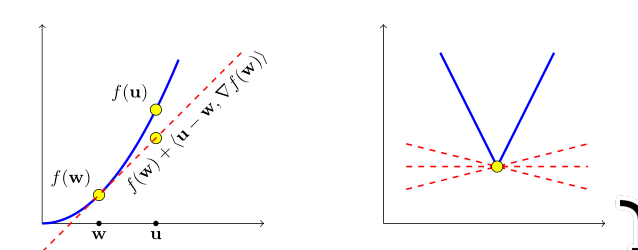
\includegraphics[width=0.6\textwidth]{figures/SubGradient.png}
  \end{itemize}
  
\end{frame}


\begin{frame}{Example Generalized Online Gradient Descent}
  Consider the $\ell_2$ setup where the functions $f_1,f_2,\ldots$ are convex (but not necessarily differentiable).
  Let $\eta$ be the learning rate.
\[
  \mathred{w_{t+1} = w_t - \eta z_t,\;\;
    z_t \in \partial f_t(w_t)}
\]
Identical to FTRL with regularization: $\mathred{R(w) = \frac{1}{2\eta}\|w\|_2^2}$

{\bf Regret bound on OGD:} From FTRL theorem:
\begin{align*}
\mathred{\text{Regret}} &\mathred{\leq \frac{\|u\|^2}{2\eta} + \eta \sum_{t=1}^T \|z_t\|^2} \\
&\mathred{\leq \frac{B^2}{2\eta} + \eta T L^2}
\end{align*}
\end{frame}


\begin{frame}{Gradient based Online Mirror Descent (OMD)}
\textbf{parameter:} a link function \( g : \mathbb{R}^d \to S \)

\textbf{initialize:} \( \textcolor{mathcolor}{\theta_1 = 0} \)

\textbf{for} \( t = 1,2,\dots \)
\begin{itemize}
    \item \textbf{project} \( \mathbf{w}_t = \textcolor{mathcolor}{ g(\theta_t) } \)
    \item \textbf{update} \( \theta_{t+1} = \textcolor{mathcolor}{ \theta_t - \mathbf{z}_t } \) where \( \mathbf{z}_t \in \textcolor{mathcolor}{ \partial f_t(\mathbf{w}_t) } \)
    \end{itemize}
    Dual Decent: Instead of minimizing \R{$f$}, minimize \R{$\nabla f$}. \\
    Convexity implies equivalence of goals.
\end{frame}

\section{Duality}

\begin{frame}
  \frametitle{Duality}
  \begin{itemize}
  \item OMD can be analyzed using elementary tools from duality.
    \item Using Duality Gives better intuition, more general analysis, tighter bounds.
  \end{itemize}
\end{frame}

\begin{frame}
\frametitle{Dual Vector Spaces}

\begin{itemize}
\item \R{$V$} is a vector space, with a norm \R{$\|v\|$}
\item \R{$U$} is the set of all linear mappings from \R{$V$} to
  \R{$V$}
  \item
  The norm of \R{$u \in U$} is defined as
  \R{$$\|u\|_* \doteq \max_{v \in V} \frac{\|u(v)\|}{\|v\|}$$}
\item \R{$V$} is equivalent to the set of all linear mappings from \R{$U$} to
  \R{$U$}.
\item \R{$U$} and \R{$V$} are dual vector spaces, with dual norms. 
\end{itemize}
\end{frame}

\begin{frame}
\frametitle{Dual Norms}
\begin{itemize}
  \item The space is always \R{$U,V = \real^n$}
  \item The linear operation is the dot product \R{$\vu \cdot \vv$}
   \item $\|u\|_*$ is the dual norm to $\|v\|$, 
\item \R{$L_2$} norm: \R{$\sqrt{\sum_{i=1}^n x_i^2}$}
\item \R{$L_1$} norm: \R{$\sum_{i=1}^n |x_i|$}
\item \R{$L_\infty$} norm: \R{$\max_i |x_i|$}
\item \R{$L_p$} norm: \R{$\paren{\sum_{i=1}^n x_i^p}^{\frac{1}{p}}$}
\item \R{$L_p,L_q$} are dual norms if \R{$p,q \geq 1, \mbox{ and }\frac{1}{p} + \frac{1}{q} = 1$}
\item \R{$L_1,L_\infty$} are dual.
\item \R{$L_2$} is self-dual. 
\end{itemize}
\end{frame}

\begin{frame}{Lipschitz condition and the dual norm}
\textbf{Lemma 2.6:}\\
Let $\mathred{f:S \to \mathbb{R}}$ be a convex function. Then, $f$ is $\mathred{L}$-Lipschitz over $S$ with respect to a norm $\mathred{\|\cdot\|}$ if and only if for all $\mathred{w \in S}$ and $\mathred{z \in \partial f(w)}$ we have:
\begin{equation*}
\mathred{\|z\|_* \leq L}
\end{equation*}
where $\mathred{\|\cdot\|_*}$ denotes the dual norm.
\end{frame}

\begin{frame}{Proof of Lemma 2.6}
\textbf{Proof:}\\
Assume that $f$ is $\mathred{L}$-Lipschitz. For any $\mathred{w \in S}$ and $\mathred{z \in \partial f(w)}$, choose $\mathred{u}$ such that $\mathred{u - w = \arg\max_{\|v\|=1} \langle v, z \rangle}$. Then,
\begin{equation*}
\mathred{\langle z, u - w \rangle = \|z\|_*}
\end{equation*}
By the sub-gradient definition,
\begin{equation*}
\mathred{f(u) - f(w) \geq \langle z, u - w \rangle = \|z\|_*}
\end{equation*}
Since $f$ is $L$-Lipschitz,
\begin{equation*}
\mathred{f(u) - f(w) \leq L \|u - w\| = L}
\end{equation*}
Combining the inequalities:
\begin{equation*}
\mathred{\|z\|_* \leq L}
\end{equation*}
For the converse, assume $\mathred{\|z\|_* \leq L}$ for all $\mathred{z \in \partial f(w)}$. Then,
\begin{equation*}
\mathred{f(u) - f(w) \leq \langle z, u - w \rangle \leq \|z\|_* \|u - w\| \leq L \|u - w\|}
\end{equation*}
Hence, $f$ is $L$-Lipschitz.
\end{frame}


\begin{frame}
\frametitle{Fenchel Duality}
\begin{itemize}
\item Suppose \R{$F:A \to \real$} is a convex function over a convex set \R{$A
    \subseteq \real^n$}.
\item The dual function to \R{$F$} is
  \R{$$
    F^*(\vu) = \sup_{\vv \in A}\paren{\vu \cdot \vv -F(\vv)}
$$}
  \item Fenchel duality Equivalent to Legendre duality for differentiable functions.

\end{itemize}
\end{frame}

\begin{frame}
  \frametitle{Visualization of the Legendre Dual}
  \begin{columns}
    \begin{column}{0.55\textwidth}
        \begin{itemize}
            \item \R{$x,y \real$}
            \item \R{$ f^*(y) = \sup_{x \in \real}\paren{xy-f(x)}$}
            \item \R{$ -f^*(y) = \inf_{x \in \real}\paren{f(x)-xy}$}
        \end{itemize}
    \end{column}
    \begin{column}{0.43\textwidth}
          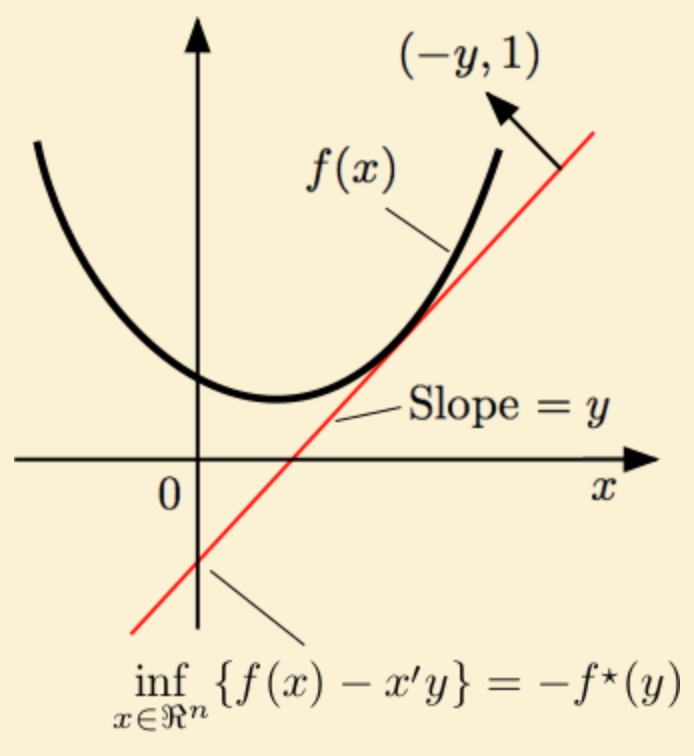
\includegraphics[width=\textwidth]{figures/Legendre-Duality.png}
    \end{column}
\end{columns}
\end{frame}

\begin{frame}
  \frametitle{Dual of Dual}
  \begin{itemize}
  \item The dual of any function is convex.
  \item if \R{$F$} is convex then \R{$F^{**} = F$}
  \end{itemize}
  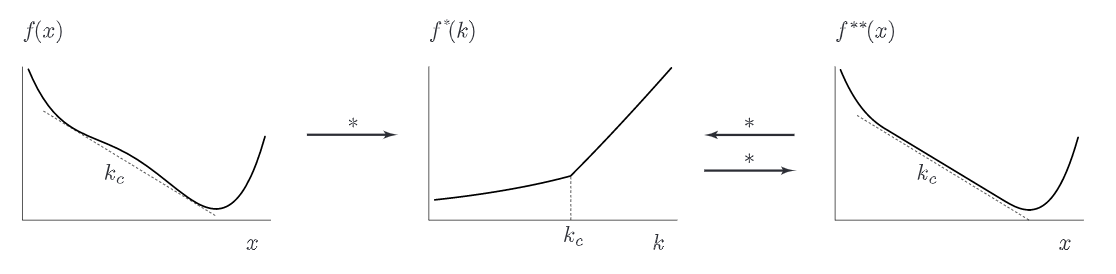
\includegraphics[width=\textwidth]{figures/FromNonConvexToConvex.png}  
\end{frame}

\begin{frame}
  \frametitle{Gradient Duality (legendre only)}
  \begin{itemize}
  \item
    If the gradient of \R{$f$} at \R{$x$} is \R{$k$} then\\
    the gradient of \R{$f^*$} at \R{$k$} is \R{$x$}
    \item In general:
  \R{$$
    \nabla F^* = \paren{\nabla F}^{-1}
    $$}
  \end{itemize}
  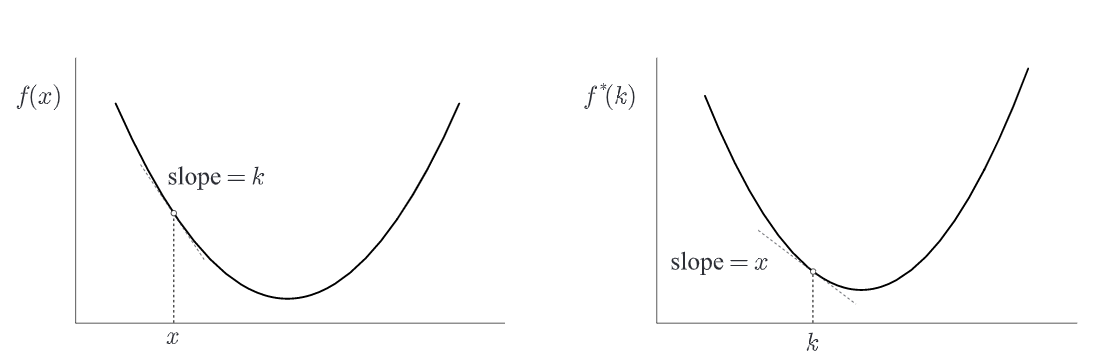
\includegraphics[width=\textwidth]{figures/SlopeDuality.png}
\end{frame}

\begin{frame}
  \frametitle{Example: Exponential Potential}
  \begin{itemize}
  \item Potential: \R{$F(\vu) = \sum_{i=1}^d e^{u_i}$}
  \item Gradient: \R{$\nabla F(\vu)_i = e^{u_i}$} or \R{$\nabla F(\vu)
      = F(\vu)$}.
  \item Dual:  \R{$F^*(\vv) = \sum_{i=1}^d v_i (\ln v_i -1)$}
  \item Gradient of dual: \R{$\nabla F^*(\vv)_i = \ln v_i $} 
  \item Note \R{$(\nabla F)^{-1} = \nabla F^*$}
   \end{itemize}
 \end{frame}

 \begin{frame}
    \frametitle{Bregman Divergence}
   \begin{columns}
     \begin{column}{0.55\textwidth}
       \begin{itemize}
       \item \R{$R(x)$} is convex and differentiable.
       \item \R{$D_R(w||u) = R(w)-(R(u) + \langle \nabla R(u) , (w-u) \rangle)$}
       \item The error term of the first order Taylor expansion around \R{$u$}
       \end{itemize}
     \end{column}
      \begin{column}{0.43\textwidth}
        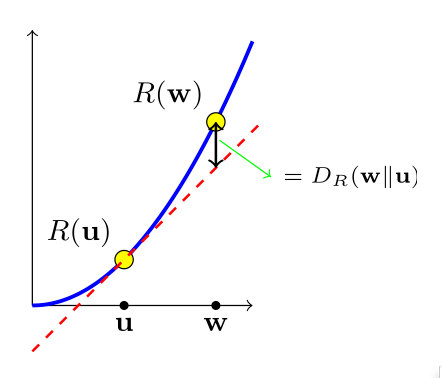
\includegraphics[width=\textwidth]{figures/BregmanDivergence.png}
      \end{column}
    \end{columns}
  \end{frame}
 
\begin{frame}
  \frametitle{Fenchel and Bregman}
  \begin{itemize}
  \item
    \R{$F$}: strictly convex with continuous first derivative.
  \item \R{$F^*$} is the Fenchel Dual of \R{$F$}
  \item \R{$D_F,D_{F^*}$} Bregman divergences wrt \R{$F,F^*$}
  \item \R{$\vu' = \nabla F(\vu)$} and \R{$\vv' = \nabla F(\vv)$}
  \item \R{$D_F(\vu,\vv)  = D_{F^*}(\vu',\vv')$}
  \end{itemize}
\end{frame}

\begin{frame}{Mirror Descent - Step 1}
\textbf{Gradient Step in Dual Space:}

\begin{equation*}
\textcolor{red}{z_{t+1} = \nabla R(w_t) - \eta \nabla f_t(w_t)}
\end{equation*}

Here, \textcolor{red}{$\nabla R(w_t)$} maps the point into the dual space.
\end{frame}

\begin{frame}{Mirror Descent - Step 2}
\textbf{Projection Back to Primal Space:}

\begin{equation*}
\textcolor{red}{w_{t+1} = \arg\min_{w \in S} D_R(w, z_{t+1})}
\end{equation*}

Where \textcolor{red}{$D_R(w, z)$} is the Bregman divergence:

\begin{equation*}
\textcolor{red}{D_R(w, z) = R(w) - R(z) - \langle \nabla R(z), w - z \rangle}
\end{equation*}

This projection ensures \textcolor{red}{$w_{t+1}$} stays within the feasible set \textcolor{red}{$S$}.
\end{frame}

\begin{frame}
  \frametitle{Mirror Descent (alternative Notation)}
  \begin{itemize}
  \item Gradient descent in dual space
    \R{$\theta_t = \theta_{t-1} - \lambda \nabla \ell_t(\theta_{t-1})$}
  \item Using duality can be rewritten as
    \R{$$\nabla \Phi^*(\vw_t) =  \nabla \Phi^*(\vw_{t-1})  - \lambda \nabla \ell_t(\vw_{t-1})$$}
  \item Projection: As \R{$\nabla \Phi$} is the inverse of \R{$\nabla \Phi^*$} we get
    \R{$$ \vw_t = \nabla \Phi \paren{\nabla \Phi^*(\vw_{t-1})  - \lambda \nabla \ell_t(\vw_{t-1})}$$}
  \end{itemize}
\end{frame}


\begin{frame}
  \frametitle{A picture of mirror descent}
\R{$$ \vw_t = \nabla \Phi \paren{\nabla \Phi^*(\vw_{t-1})  - \lambda \nabla \ell_t(\vw_{t-1})}$$}
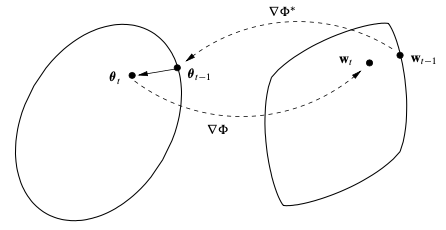
\includegraphics[width=\textwidth]{figures/MirrorDescent.png}
\end{frame}


\begin{frame}{Regret Bound for OMD}
\textbf{Lemma 2.20.} Suppose that OMD is run with a link function \( g = \nabla R^* \). Then, its regret is upper bounded by:

\[
\sum_{t=1}^{T} \textcolor{mathcolor}{ \langle \mathbf{w}_t - \mathbf{u}, \mathbf{z}_t \rangle }
\leq \textcolor{mathcolor}{ R(\mathbf{u}) - R(\mathbf{w}_1) }
+ \sum_{t=1}^{T} \textcolor{mathcolor}{ D_{R^*}(-\mathbf{z}_{1:t} \| -\mathbf{z}_{1:t-1}) }
\]

Furthermore, equality holds for the vector \( \mathbf{u} \) that minimizes \( \textcolor{mathcolor}{ R(\mathbf{u}) + \sum_t \langle \mathbf{u}, \mathbf{z}_t \rangle } \).
\end{frame}

\begin{frame}{Proof: Step 1 - Fenchel–Young Inequality}
Using the \textbf{Fenchel–Young inequality}, we have:
\[
\textcolor{mathcolor}{ R(\mathbf{u}) + \sum_{t=1}^{T} \langle \mathbf{u}, \mathbf{z}_t \rangle }
= R(\mathbf{u}) - \langle \mathbf{u}, -\mathbf{z}_{1:T} \rangle
\geq \textcolor{mathcolor}{ -R^*(-\mathbf{z}_{1:T}) }.
\]

Equality holds for \( \mathbf{u} \) that maximizes \( \langle \mathbf{u}, -\mathbf{z}_{1:T} \rangle - R(\mathbf{u}) \), hence minimizing \( R(\mathbf{u}) + \langle \mathbf{u}, \mathbf{z}_{1:T} \rangle \).
\end{frame}

\begin{frame}{Proof: Step 2 - Bregman Divergence}
Since \( \mathbf{w}_t = \nabla R^*(-\mathbf{z}_{1:t-1}) \) and using the definition of the Bregman divergence, we rewrite:

\[
\textcolor{mathcolor}{ -R^*(-\mathbf{z}_{1:T}) }
= -R^*(0) - \sum_{t=1}^{T} \textcolor{mathcolor}{ (R^*(-\mathbf{z}_{1:t}) - R^*(-\mathbf{z}_{1:t-1})) }.
\]

Rearranging, we get:
\[
= \textcolor{mathcolor}{ -R^*(0) + \sum_{t=1}^{T} (\langle \mathbf{w}_t, \mathbf{z}_t \rangle - D_{R^*}(-\mathbf{z}_{1:t} \| -\mathbf{z}_{1:t-1})) }.
\]
\end{frame}

\begin{frame}{Final Step}
\textbf{Note:} Since
\[
\textcolor{mathcolor}{ R^*(0) = \max_{\mathbf{w}} \langle 0, \mathbf{w} \rangle - R(\mathbf{w}) = - \min_{\mathbf{w}} R(\mathbf{w}) = -R(\mathbf{w}_1) },
\]
combining all the above, we conclude the proof. \(\square\)
\end{frame}
%%%%%
\section{Algorithms for specific potentials}

\iffalse
  \begin{frame}
  \frametitle{Polynomial Potential}
  \begin{itemize}
  \item Potential: \R{$\Phi_p(\vu) = \frac{1}{2} \|\vu\|_p^2= \frac{1}{2} \paren{\sum_{i=1}^d
        u_i^p}^{2/p}$}
  \item Dual Potential \R{$\Phi_p^* = \Phi_q$} Where
    \R{$\frac{1}{p}+\frac{1}{q} = 1$}
  \item Euclidean norm: \R{$q=p=2$}
  \item Suppose the sequence of examples
    \R{$(\vx_1,y_1),\ldots,(\vx_T,y_T)$} satisfies \R{$\| \vx_t \|_p
      \leq X_p$} for all \R{$1 \leq t \leq T$}
  \item Suppose we use the dual descend algorithm for the potential
    function \R{$\Phi_p$} and the learning rate \R{$\lambda =
      \frac{2 \epsilon}{(p-1) X_p^2}$} for some \R{$0<\epsilon<1$}
  \item \B{Loss Bound}:\\
    \R{$L_{A,T}  \leq \frac{L_T(\vu)}{1-\epsilon} + \frac{\| \vu
        \|_q^2}{\epsilon (1-\epsilon)}\times \frac{(p-1)X_p^2}{4}$}
  \end{itemize}
\end{frame}
\fi

\begin{frame}{OMD for $\ell_2$}
  \begin{itemize}
  \item Problem: OCO where \R{$\forall z \in \partial f(x) $} \R{$\|z\|_2\leq X_2$}
  \item The dual norm for the weights is \R{$\|w\|_2$}
  \item We use the dual descend algorithm for the half quadratic regularizer 
  \item Regularizer: \R{$\Phi(\vu) = \frac{1}{2}\|\vu\|_2^2$}
  \item Legendre Dual Regularizer \R{$\Phi^*(\vu) = \frac{1}{2}\|\vu\|_2^2$}
    \item \textbf{Gradient Mapping:} \textcolor{red}{$\nabla R(w) = w$}
\item Gradient step: $\textcolor{red}{z_{t+1} = w_t - \eta \nabla f_t(w_t)}$

    \end{itemize}
\end{frame}

\begin{frame}{Projection Step for \(\ell_2\) Norm}
\textbf{Bregman Divergence:}

\begin{equation*}
\textcolor{red}{D_R(w, z) = \frac{1}{2} \|w - z\|_2^2}
\end{equation*}

\textbf{Projection Back to Primal Space:}

\begin{equation*}
\textcolor{red}{w_{t+1} = \Pi_S (z_{t+1}) = \arg\min_{w \in S} \frac{1}{2} \|w - z_{t+1}\|_2^2}
\end{equation*}

Where \textcolor{red}{$\Pi_S$} denotes the Euclidean projection onto the feasible set \textcolor{red}{$S$}.
\end{frame}

\begin{frame}{Final Update Rule for \(\ell_2\) Norm}
Combining both steps, the final update rule becomes:

\begin{equation*}
\textcolor{red}{w_{t+1} = \Pi_S \left( w_t - \eta \nabla f_t(w_t) \right)}
\end{equation*}

This is equivalent to the standard \textbf{Projected Gradient Descent} for the \(\ell_2\) norm.
\end{frame}
\begin{frame}{Optimal Tuning for \(\eta\) and Regret Bound}
\textbf{Regret Bound:}

\begin{equation*}
\textcolor{red}{\text{Regret}_T(u) \leq \frac{\|u\|_2^2}{2\eta} + \frac{\eta}{2} \sum_{t=1}^T \|\nabla f_t(w_t)\|_2^2}
\end{equation*}

Assuming \textcolor{red}{$\|u\|_2 \leq B$} and \textcolor{red}{$\|\nabla f_t(w_t)\|_2 \leq L$}, this simplifies to:

\begin{equation*}
\textcolor{red}{\text{Regret}_T(u) \leq \frac{B^2}{2\eta} + \frac{\eta L^2 T}{2}}
\end{equation*}

\textbf{Optimal \(\eta\):}

\begin{equation*}
\textcolor{red}{\eta^* = \frac{B}{L\sqrt{T}}}
\end{equation*}

\textbf{Resulting Regret Bound:}

\begin{equation*}
\textcolor{red}{\text{Regret}_T(u) \leq B L \sqrt{T}}
\end{equation*}
\end{frame}

\begin{frame}
  \frametitle{$\ell_{\infty}$ OMD}
  \begin{itemize}
  \item Problem: OCO where \R{$\forall z \in \partial f(x) $} \R{$\|z\|_\infty \leq X_\infty$}
  \item The dual norm for the weights is \R{$\|w\|_1$}
  \item Suppose we use the dual descend algorithm for the exponential regularizer
  \item Regularizer: \R{$\Phi(\vu) = \frac{1}{\eta} \ln \sum_{i=1}^d e^{\eta u_i}$}
  \item Legendre Dual Regularizer \R{$\Phi^*(\vu) = \sum_{i=1}^d u_i (\ln u_i -1)$}
  \end{itemize}
\end{frame}
\begin{frame}
  \begin{itemize}
  \item Weight update:
    \R{$$\vw_t = \nabla \Phi \paren{\nabla \Phi^*(\vw_{t-1})  - \lambda \nabla \ell_t(\vw_{t-1})}$$}
    
  \item Unnormalized exponentiated gradient: \R{$$w_{i,t}=w_{i,t-1}e^{-\lambda \nabla \ell_t(w_i-1)}$$}
  \item Normalized exponentiated gradient:
    \R{$$w_{i,t}=\frac{w_{i,t-1}e^{-\lambda \nabla \ell_t(w_i-1)}}
      {\sum_{j=1}^d w_{j,t-1}e^{-\lambda \nabla \ell_t(w_j-1)}}$$}
  \end{itemize}
\end{frame}

\begin{frame}
  \begin{itemize}
  \item Normalization corresponds to projection on the simplex
    using the Bregman divergence according to $\Phi^*$. 
  \item The dual descend algorithm for the exponential regularizer
    function \R{$\Phi$} and the learning rate \R{$\lambda =
      \frac{2 \epsilon}{X_{\infty}^2}$}  for some \R{$0<\epsilon<1$}
  \item yields \B{Loss Bound}:\\
    \R{$$L_{A,T}  \leq \frac{L_T(\vu)}{1-\epsilon} + \frac{X_\infty^2
        \ln d}{2 \epsilon (1-\epsilon)}$$}
  \end{itemize}
\end{frame}
\end{small}
\end{document}

%%% Local Variables:
%%% mode: latex
%%% TeX-master: t
%%% End:
